The second question of the survey asks Android developers the programming language or programming languages they use to develop Android applications. As mentioned in section \ref{section:2.1.2}, different programming languages can be used while developing Android applications. Java and Kotlin programming languages are among the options offered to answer the second question.
\begin{figure}[ht!]
    \centering
    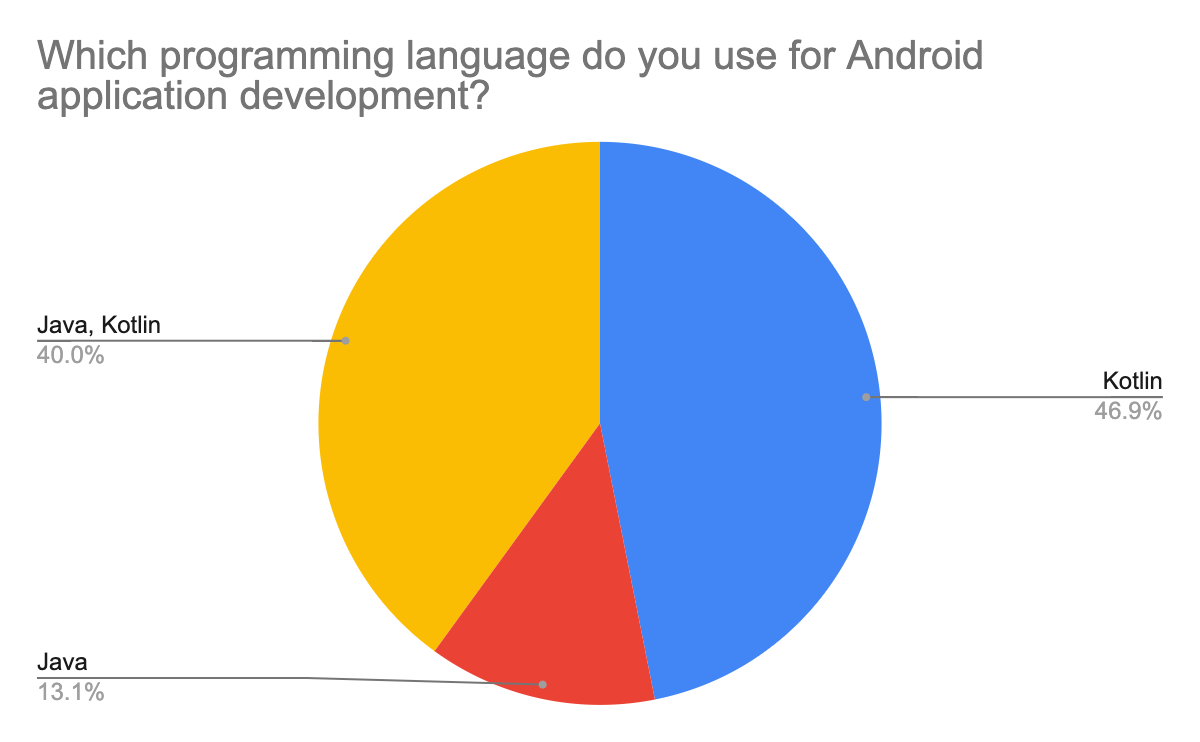
\includegraphics[scale=0.3]{figures/survey_q2_programming_language.png}
    \caption{Programming languages results}
    \label{fig:programming_languages}
\end{figure}

Fig. \ref{fig:programming_languages} presents the Android developers' trends regarding the programming language they use while developing "Native" Android applications. Around 47\% of the Android developers surveyed seem to use the Kotlin programming language. 40\% of the participants use Java and Kotlin together, while only 13.1\% use the Java programming language.